\documentclass{beamer}
\usepackage{natbib}
\usepackage{amsmath}
\usetheme{Madrid}
\setbeamertemplate{caption}[numbered]
\newcommand{\bs}[1]{\boldsymbol{#1}}
\newcommand{\info}{\mathcal{I}}
\setbeamertemplate{frametitle continuation}[from second][]


\title[bla]{bla bla}

\author[Yulia Sidi]{{\footnotesize Yulia Sidi}}
%\institute[HSPH]{}
\institute[UConn]{Applied General Exam \\ 
Department of Statistics, University of Connecticut}
\date[January 14, 2019]{{\scriptsize January 14, 2019}}


% Let's get started
\begin{document}

\begin{frame}
\titlepage
\end{frame}

\AtBeginSection[]{\begin{frame}{Outline}
  \tableofcontents[hideallsubsections, currentsection]
\end{frame}}

% Section and subsections will appear in the presentation overview
% and table of contents.
\section{Introduction}

\subsection{WRITE INTRO}

\begin{frame}{}{}
\end{frame}

\section{Results}


\begin{frame}{Geographic Variation in Gender Gaps- Replicated}
\begin{columns}
	
	\begin{column}{0.52\textwidth}
		\vspace{\topsep}
		\begin{figure}
		\vspace{-0.5cm}	
		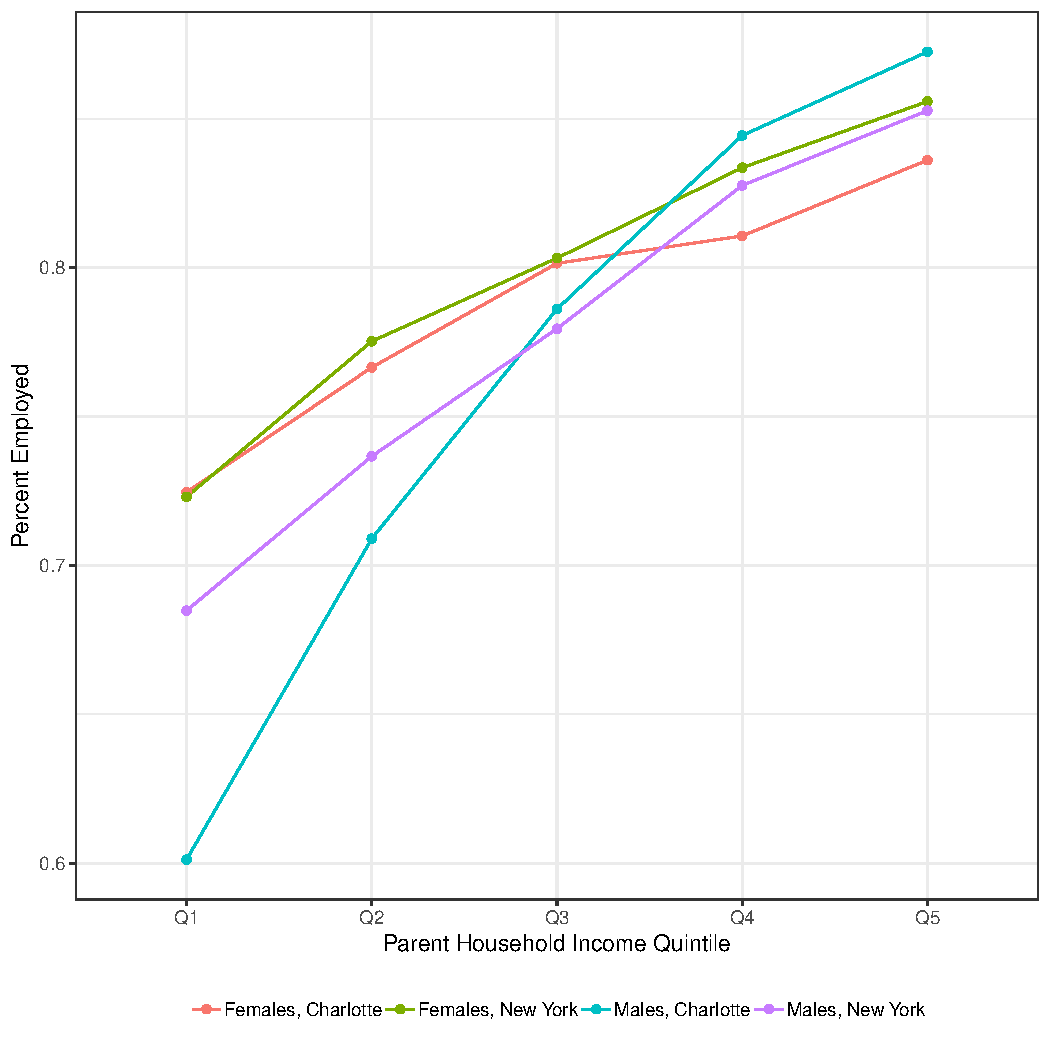
\includegraphics[width=\columnwidth]{../fig2.pdf}
		\caption{{\scriptsize Children’s Employment Rates by Gender and Parent Income Quintile:
			New York vs. Charlotte CZs}}
		\end{figure}	
\end{column}
	
	\begin{column}{0.4\textwidth}
				\vspace{-2.5cm}	
		\begin{itemize}
			\item Among females, percent employment is similar between the CZs across the distribution of parent household income.
			\item The gaps between females and males are more pronounced in Charlotte for low-income parents.
		\end{itemize}
	\end{column}
	
\end{columns}
\end{frame}


\begin{frame}{Geographic Variation in Gender Gaps}
\begin{columns}
	
	\begin{column}{0.52\textwidth}
		\vspace{\topsep}
		\begin{figure}
			\vspace{-0.5cm}	
			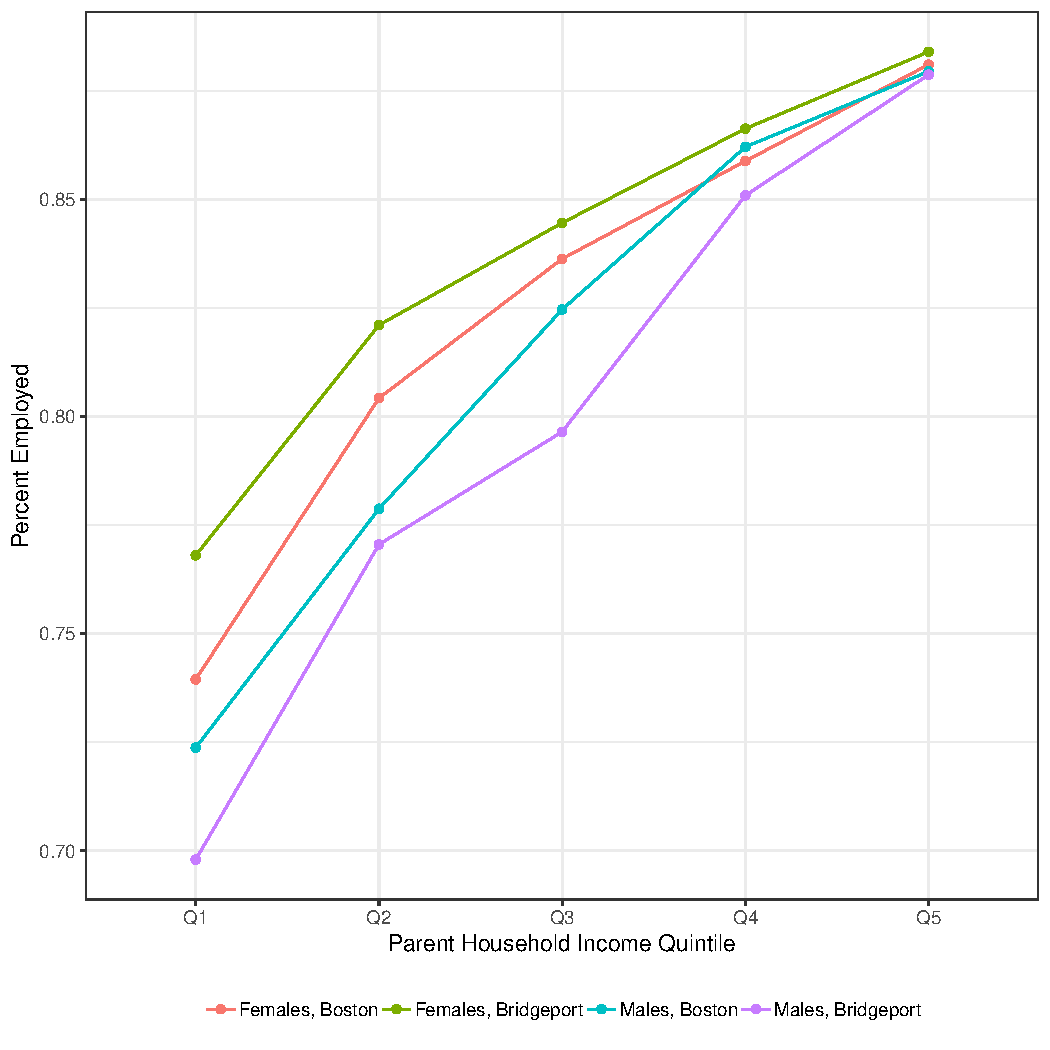
\includegraphics[width=\columnwidth]{../fig2_new.pdf}
			\caption{{\scriptsize Children’s Employment Rates by Gender and Parent Income Quintile:
					Boston vs. Bridgeport CZs}}
		\end{figure}	
	\end{column}
	
	\begin{column}{0.4\textwidth}
		\vspace{-2.5cm}	
		\begin{itemize}
			\item Among females, percent employment is slightly higher in Bridgeport across the parent income distribution. 
			\item The gaps between females and males are much more pronounced in Bridgeport for low/middle-income parents.
		\end{itemize}
	\end{column}
	
\end{columns}
\end{frame}

\begin{frame}{Geographic Variation in Gender Gaps}
\begin{columns}
	
	\begin{column}{0.52\textwidth}
		\vspace{\topsep}
		\begin{figure}
			\vspace{-0.5cm}	
			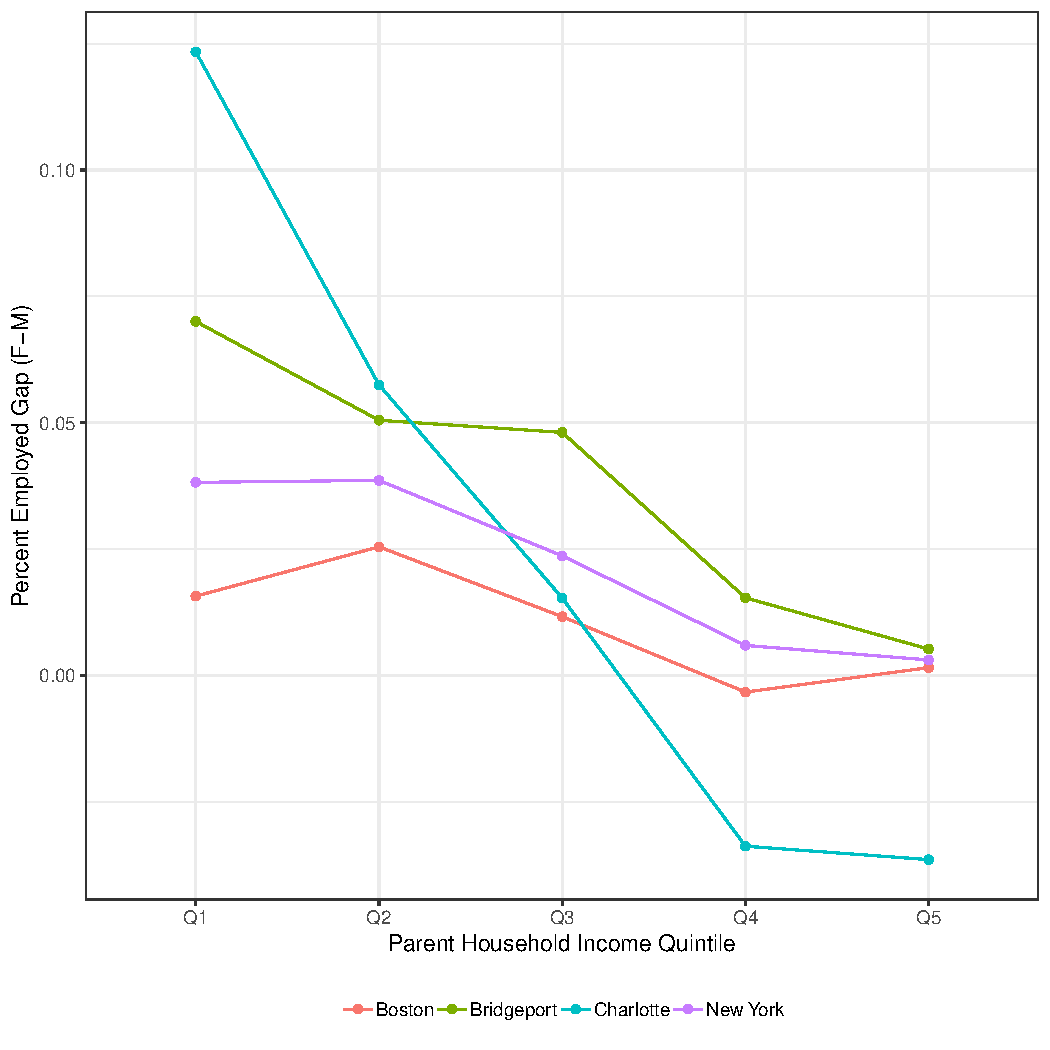
\includegraphics[width=\columnwidth]{../fig_ys.pdf}
			\caption{{\scriptsize Gender Gaps in Children’s Employment Rates by Parent Income Quintile:
					New-York/Charlotte/Boston/Bridgeport CZs}}
		\end{figure}	
	\end{column}
	
	\begin{column}{0.4\textwidth}
		\vspace{-2.5cm}	
		\begin{itemize}
			\item The gender gaps change more extremely in Charlotte. 
			\item In Boston, New-York and Bridgeport the gaps disappear with higher parent income, which is not the case for Charlotte.
		\end{itemize}
	\end{column}
	
\end{columns}
\end{frame}

\begin{frame}{Geographic Variation in Gender Gaps- Conclusion}
Gender gaps in low-income families vary geographically.
\end{frame}


\begin{frame}
\begin{center}
\huge{Thank you!}
\end{center}
\end{frame}
\end{document}

